\subsection{Implementation}

Only a small change to the calling code of the fft, as well as the way the recursive calls are made is needed to adapt the recursive implementation to use OpenMP.

\textbf{Calling Code:}
\begin{lstlisting}
  #pragma omp parallel shared(timeUsed, in, out, len)
  {
    #pragma omp single
    {
      fft(in, out, len);
    }
  }
\end{lstlisting}

\textbf{Recursive Calls:}
\begin{lstlisting}
  #pragma omp task final(((len/2)/step) < 1024)
  {fft_help(dc2, dc1, len, step*2);}
  #pragma omp task final(((len/2)/step) < 1024)
  {fft_help(dc2+step, dc1+step, len, step*2);}
  #pragma omp taskwait
\end{lstlisting}

\textbf{Description of #pragma statements}
\begin{lstlisting}
#pragma omp parallel shared(timeUsed, in, out, len)
\end{lstlisting}
Defines a parallel section which will be executed by all existing threads and tells OpenMP that the variables timeUsed, in, out and len should be shared amongst all threads.

\begin{lstlisting}
#pragma omp single
\end{lstlisting}
Defines a section which will only be executed by a single thread. This ensures that only one thread executes the recursive calls and creates the tasks. Otherwise the same task will be created by multiple threads.

\begin{lstlisting}
#pragma omp task final(((len/2)/step) < 1024)
\end{lstlisting}
Defines a task, which will be put into a taskpool where it is available for execution by another thread. If the condition in the final clause evaluates to true,
this task, and all further tasks created by it, will be executed immediately by the encountering thread. This reduces the overhead of putting the task into the pool.

\pagebreak
\begin{lstlisting}
#pragma omp taskwait
\end{lstlisting}
Tells OpenMP to wait here until the two tasks created above are completed. This is needed to ensure the correct order of execution for the Fast Fourier Transform.

\subsection{Performance}
\subsection{Speedup}
The following graph shows the speedup relative to our fastest sequential implementation.
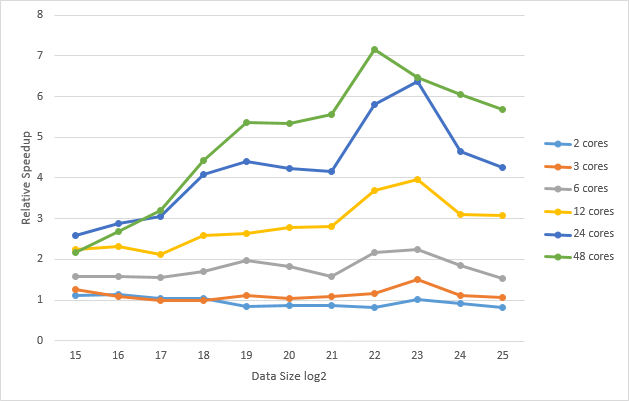
\includegraphics{rec_openmp_speedup.png}

What we can see here is that the speedup for larger amount of cores depends especially on the amount of data supplied.
The drop in speedup after about 2^{23}$ is probably due to the rising overhead associated with managing the tasks created by the program.
